\documentclass[letter]{article}
\renewcommand{\baselinestretch}{1.25}

\usepackage[margin=1in]{geometry}
\usepackage{physics}
\usepackage{amsmath, mathtools}
\numberwithin{equation}{section}
\usepackage{amssymb}
\usepackage{graphicx}
\usepackage{hyperref}
\usepackage{empheq}
\usepackage{pdfpages}

% MATLAB Formatting Code
\usepackage[numbered,framed]{matlab-prettifier}
\lstset{style=Matlab-editor,columns=fullflexible}
\renewcommand{\lstlistingname}{Script}
\newcommand{\scriptname}{\lstlistingname}

\allowdisplaybreaks

%opening
\title{MECH 6323 - HW 2}
\author{Jonas Wagner}
\date{2022, Febuary 14}

\begin{document}	

\maketitle

\tableofcontents

%----------------------------------------------------------------------------
\newpage
\section{Problem 1}
Consider the negative feedback interconnection:
\begin{figure}[ht]
	\centering
	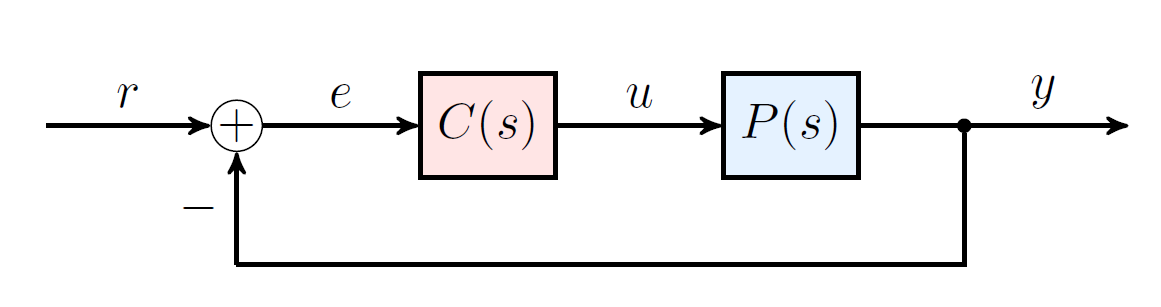
\includegraphics[width=0.5\textwidth]{figs/pblm1.png}
\end{figure}

\subsection{(a)}
\textbf{Problem:} 
If possible, give an example of $P$ and $C$ transfer functions such that $\frac{1}{1+PC}$ and $\frac{P}{1+PC}$ are stable, but $\frac{C}{1+PC}$ is not.

\textbf{Solution:}
\[
	P(s) = (s+1) (s-1)
\]\[
	C(s) = \frac{1}{(s-1)}
\]
These then produces the two following stable transfer functions:
\[
	\frac{1}{1+PC} = \frac{1}{s+2}
\]\[
	\frac{P}{1+PC} = \frac{(s+1)(s-1)}{(s+2)}
\]
However, then this transfer function is unstable:
\[
	\frac{C}{1+PC} = \frac{1}{(s-1)(s+2)}
\]

\subsection{(b)}
\textbf{Problem:} 
If possible, give an example of $P$ and $C$ transfer functions such that $\frac{P}{1+PC}$ and $\frac{C}{1+PC}$ are stable, but $\frac{1}{1+PC}$ is not.

\textbf{Solution:}
This is imposable to do for just a Transfer Function if assuming that pole-zero cancellations on the right-half plane are legitimate.
If this is not the case, there are a myriad of cases in which this would be possible to construct a case where $1+PC$ is unstable and this is due to cancellations that exist in the right-half plane, but this simple solution is not true under the previous assumption.

\newpage
\subsection{(c)}
\textbf{Problem:} 
If possible, give an example of $P$ and $C$ transfer functions such that $\frac{1}{1+PC}$ and $\frac{C}{1+PC}$ are stable, but $\frac{P}{1+PC}$ is not.

\textbf{Solution:}
\[
	P(s) = \frac{1}{(s-1)}
\]\[
	C(s) = (s+1) (s-1)
\]
These then produces the two following stable transfer functions:
\[
	\frac{1}{1+PC} = \frac{1}{s+2}
\]\[
	\frac{C}{1+PC} = \frac{(s+1)(s-1)}{(s+2)}
\]
However, then this transfer function is unstable:
\[
	\frac{P}{1+PC} = \frac{1}{(s-1)(s+2)}
\]


\newpage
\section{Problem 2}
\subsection{(a)}
\[
	G = \cfrac{
		100 s + 100
	}{
		s^2 + 110s + 1000
	}
	= \cfrac{
		100 (s+1)
	}{
		(s+100) (s+10)
	}
\]
\begin{enumerate}
	\item Zeros:
	\begin{enumerate}
		\item $z_1 = -1$
	\end{enumerate}
	\item Poles:
	\begin{enumerate}
		\item $p_1 = -100$
		\item $p_2 = -10$
	\end{enumerate}
	\item Gain:
	\begin{enumerate}
		\item $K = 100$
	\end{enumerate}
\end{enumerate}

\begin{figure}[h!]
	\centering
	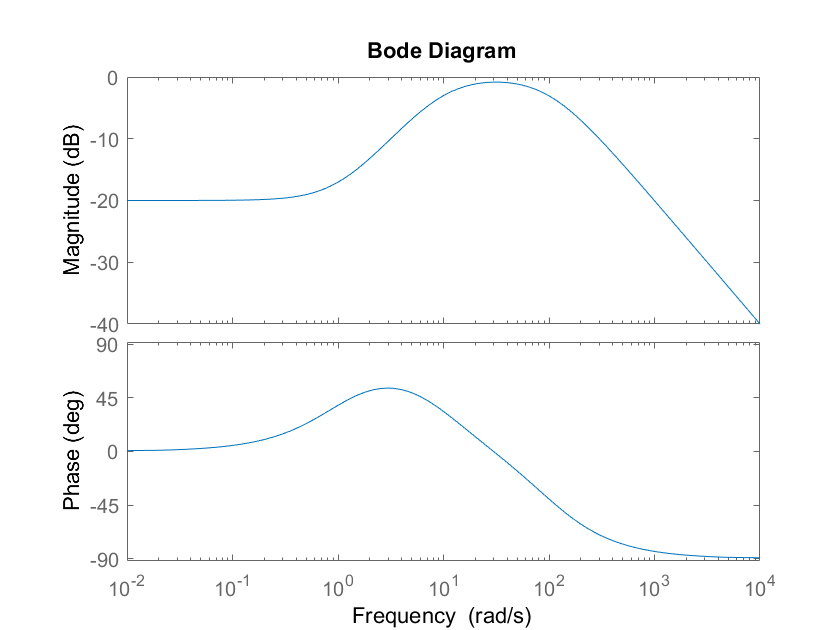
\includegraphics[width=\textwidth]{figs/pblm2a.png}
\end{figure}

\newpage
\subsection{(b)}
\[
	G = \cfrac{
		10 s
	}{
		s^2 + 3s
	}
	= \cfrac{
		10 s
	}{
		s (s + 3)
	}
\]
\begin{enumerate}
	\item Zeros:
	\begin{enumerate}
		\item $z_1 = 0$
	\end{enumerate}
	\item Poles:
	\begin{enumerate}
		\item $p_1 = 0$
		\item $p_2 = -3$
	\end{enumerate}
	\item Gain:
	\begin{enumerate}
		\item $K = 10$
	\end{enumerate}
\end{enumerate}

\begin{figure}[h!]
	\centering
	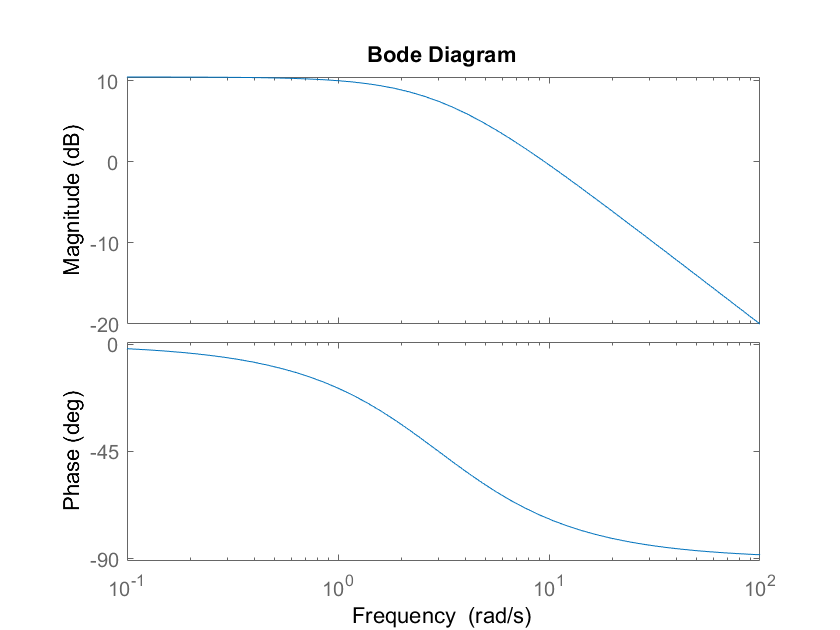
\includegraphics[width=\textwidth]{figs/pblm2b.png}
\end{figure}


\newpage
\subsection{(c)}
\[
	G = \cfrac{
		-100 s
	}{
		(s+1)^2 (s+10)
	}
\]
\begin{enumerate}
	\item Zeros:
	\begin{enumerate}
		\item $z_1 = 0$
	\end{enumerate}
	\item Poles:
	\begin{enumerate}
		\item $p_{1,2} = -1$
		\item $p_3 = -10$
	\end{enumerate}
	\item Gain:
	\begin{enumerate}
		\item $K = -100$
	\end{enumerate}
\end{enumerate}

\begin{figure}[h!]
	\centering
	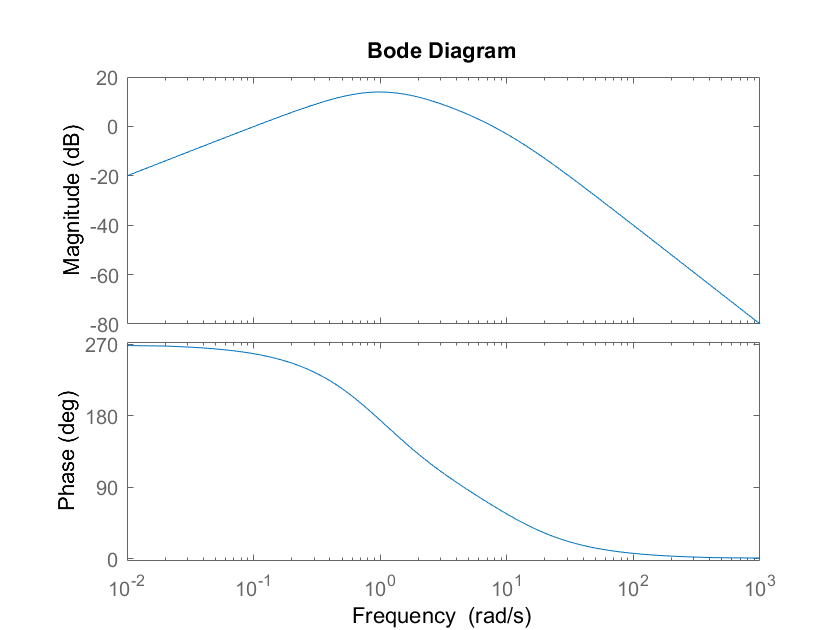
\includegraphics[width=\textwidth]{figs/pblm2c.png}
\end{figure}


\newpage
\subsection{(d)}
\[
	G = \cfrac{
		30 (s + 10)
	}{
		s^2 + 3s + 50
	}
	= \cfrac{
		30 (s+10)
	}{
		(s + 1.5 - j6.91) (s + 1.5 + j6.91)
	}
\]
\begin{enumerate}
	\item Zeros:
	\begin{enumerate}
		\item $z_1 = -10$
	\end{enumerate}
	\item Poles:
	\begin{enumerate}
		\item $p_{1,2} = -1.5 \pm j 6.91$
	\end{enumerate}
	\item Gain:
	\begin{enumerate}
		\item $K = 30$
	\end{enumerate}
\end{enumerate}

\begin{figure}[h!]
	\centering
	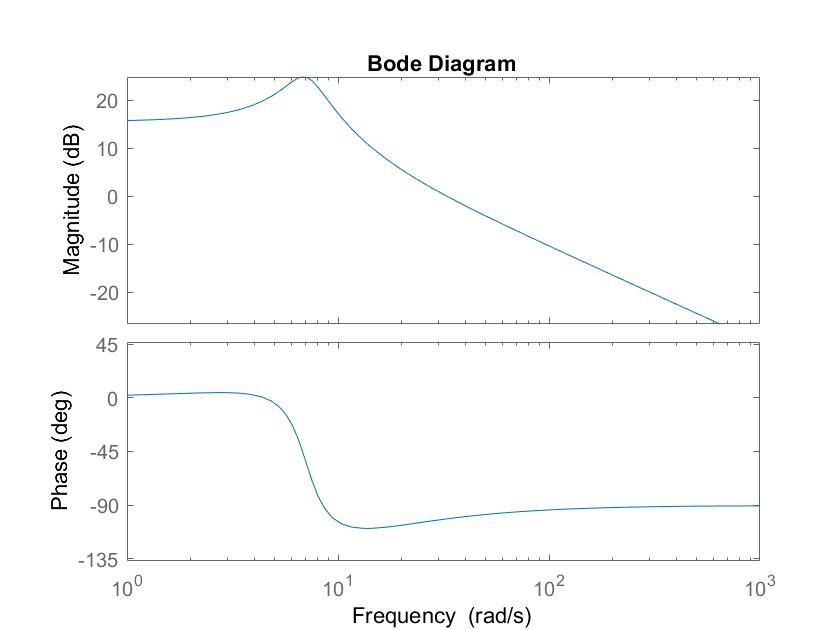
\includegraphics[width=\textwidth]{figs/pblm2d.png}
\end{figure}



\newpage
\subsection{(e)}
\[
	G = \cfrac{
		4 (s^2 + s + 25)
	}{
		s^3 + 100s^2
	}
	= \cfrac{
		4 (s + 0.5 + j 4.9749) (s + 0.5 - j 4.9749)
	}{
		s^2 (s+100)
	}
\]
\begin{enumerate}
	\item Zeros:
	\begin{enumerate}
		\item $z_{1,2} = -0.5 \pm j 4.9749$
	\end{enumerate}
	\item Poles:
	\begin{enumerate}
		\item $p_{1,2} = 0$
		\item $p_3 = -100$
	\end{enumerate}
	\item Gain:
	\begin{enumerate}
		\item $K = 4$
	\end{enumerate}
\end{enumerate}

\begin{figure}[h!]
	\centering
	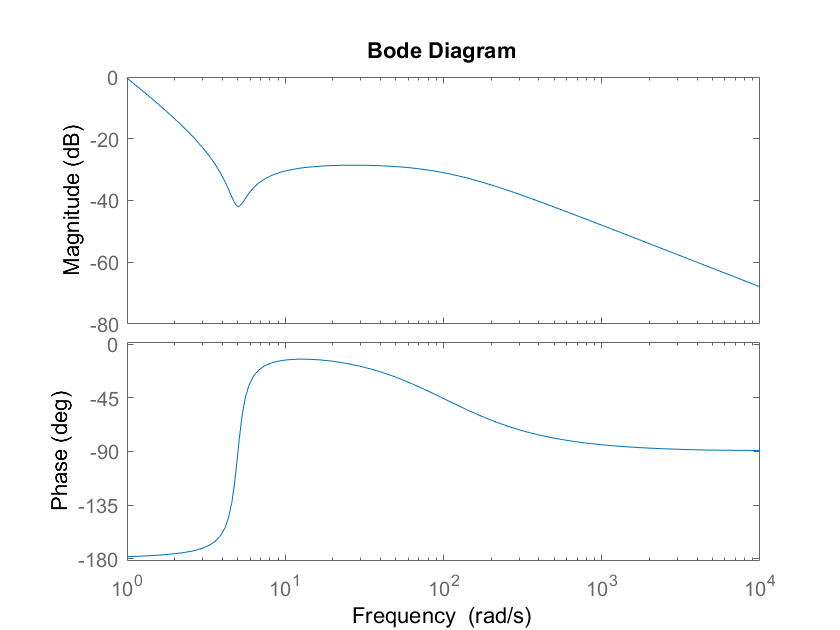
\includegraphics[width=\textwidth]{figs/pblm2e.png}
\end{figure}



\newpage
\subsection{(f)}
\[
	G = \cfrac{
		10
	}{
		s^2 (1 + 0.2s) (1 + 0.5s)
	}
	= \cfrac{
		100
	}{
		s^2 (s+5)(s+2)
	}
\]
\begin{enumerate}
	\item Zeros: NA
	\item Poles:
	\begin{enumerate}
		\item $p_{1,2} = 0$
		\item $p_3 = -5$
		\item $p_4 = -2$
	\end{enumerate}
	\item Gain:
	\begin{enumerate}
		\item $K = 100$
	\end{enumerate}
\end{enumerate}

\begin{figure}[h!]
	\centering
	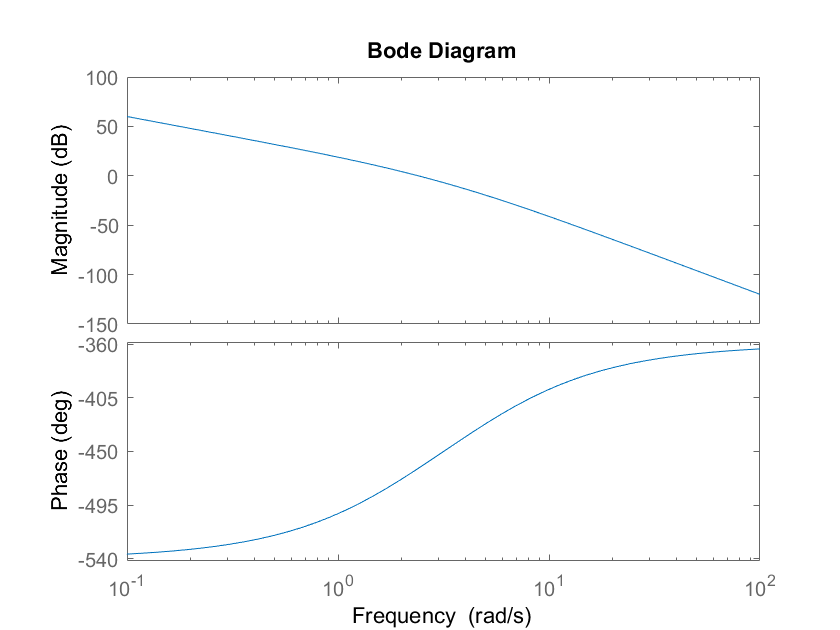
\includegraphics[width=\textwidth]{figs/pblm2f.png}
\end{figure}

\newpage
\section{Problem 3}
\textbf{Problem:}
For each of the bode plots:
\begin{enumerate}
	\item Determine the breakpoints and the transfer function.
	\item Determine the gain cross-over frequency $\omega_c$ and the phase cross-over frequency $\omega_{180}$.
\end{enumerate}

\subsection{Bode Plot 1:}
\begin{figure}[ht]
	\centering
	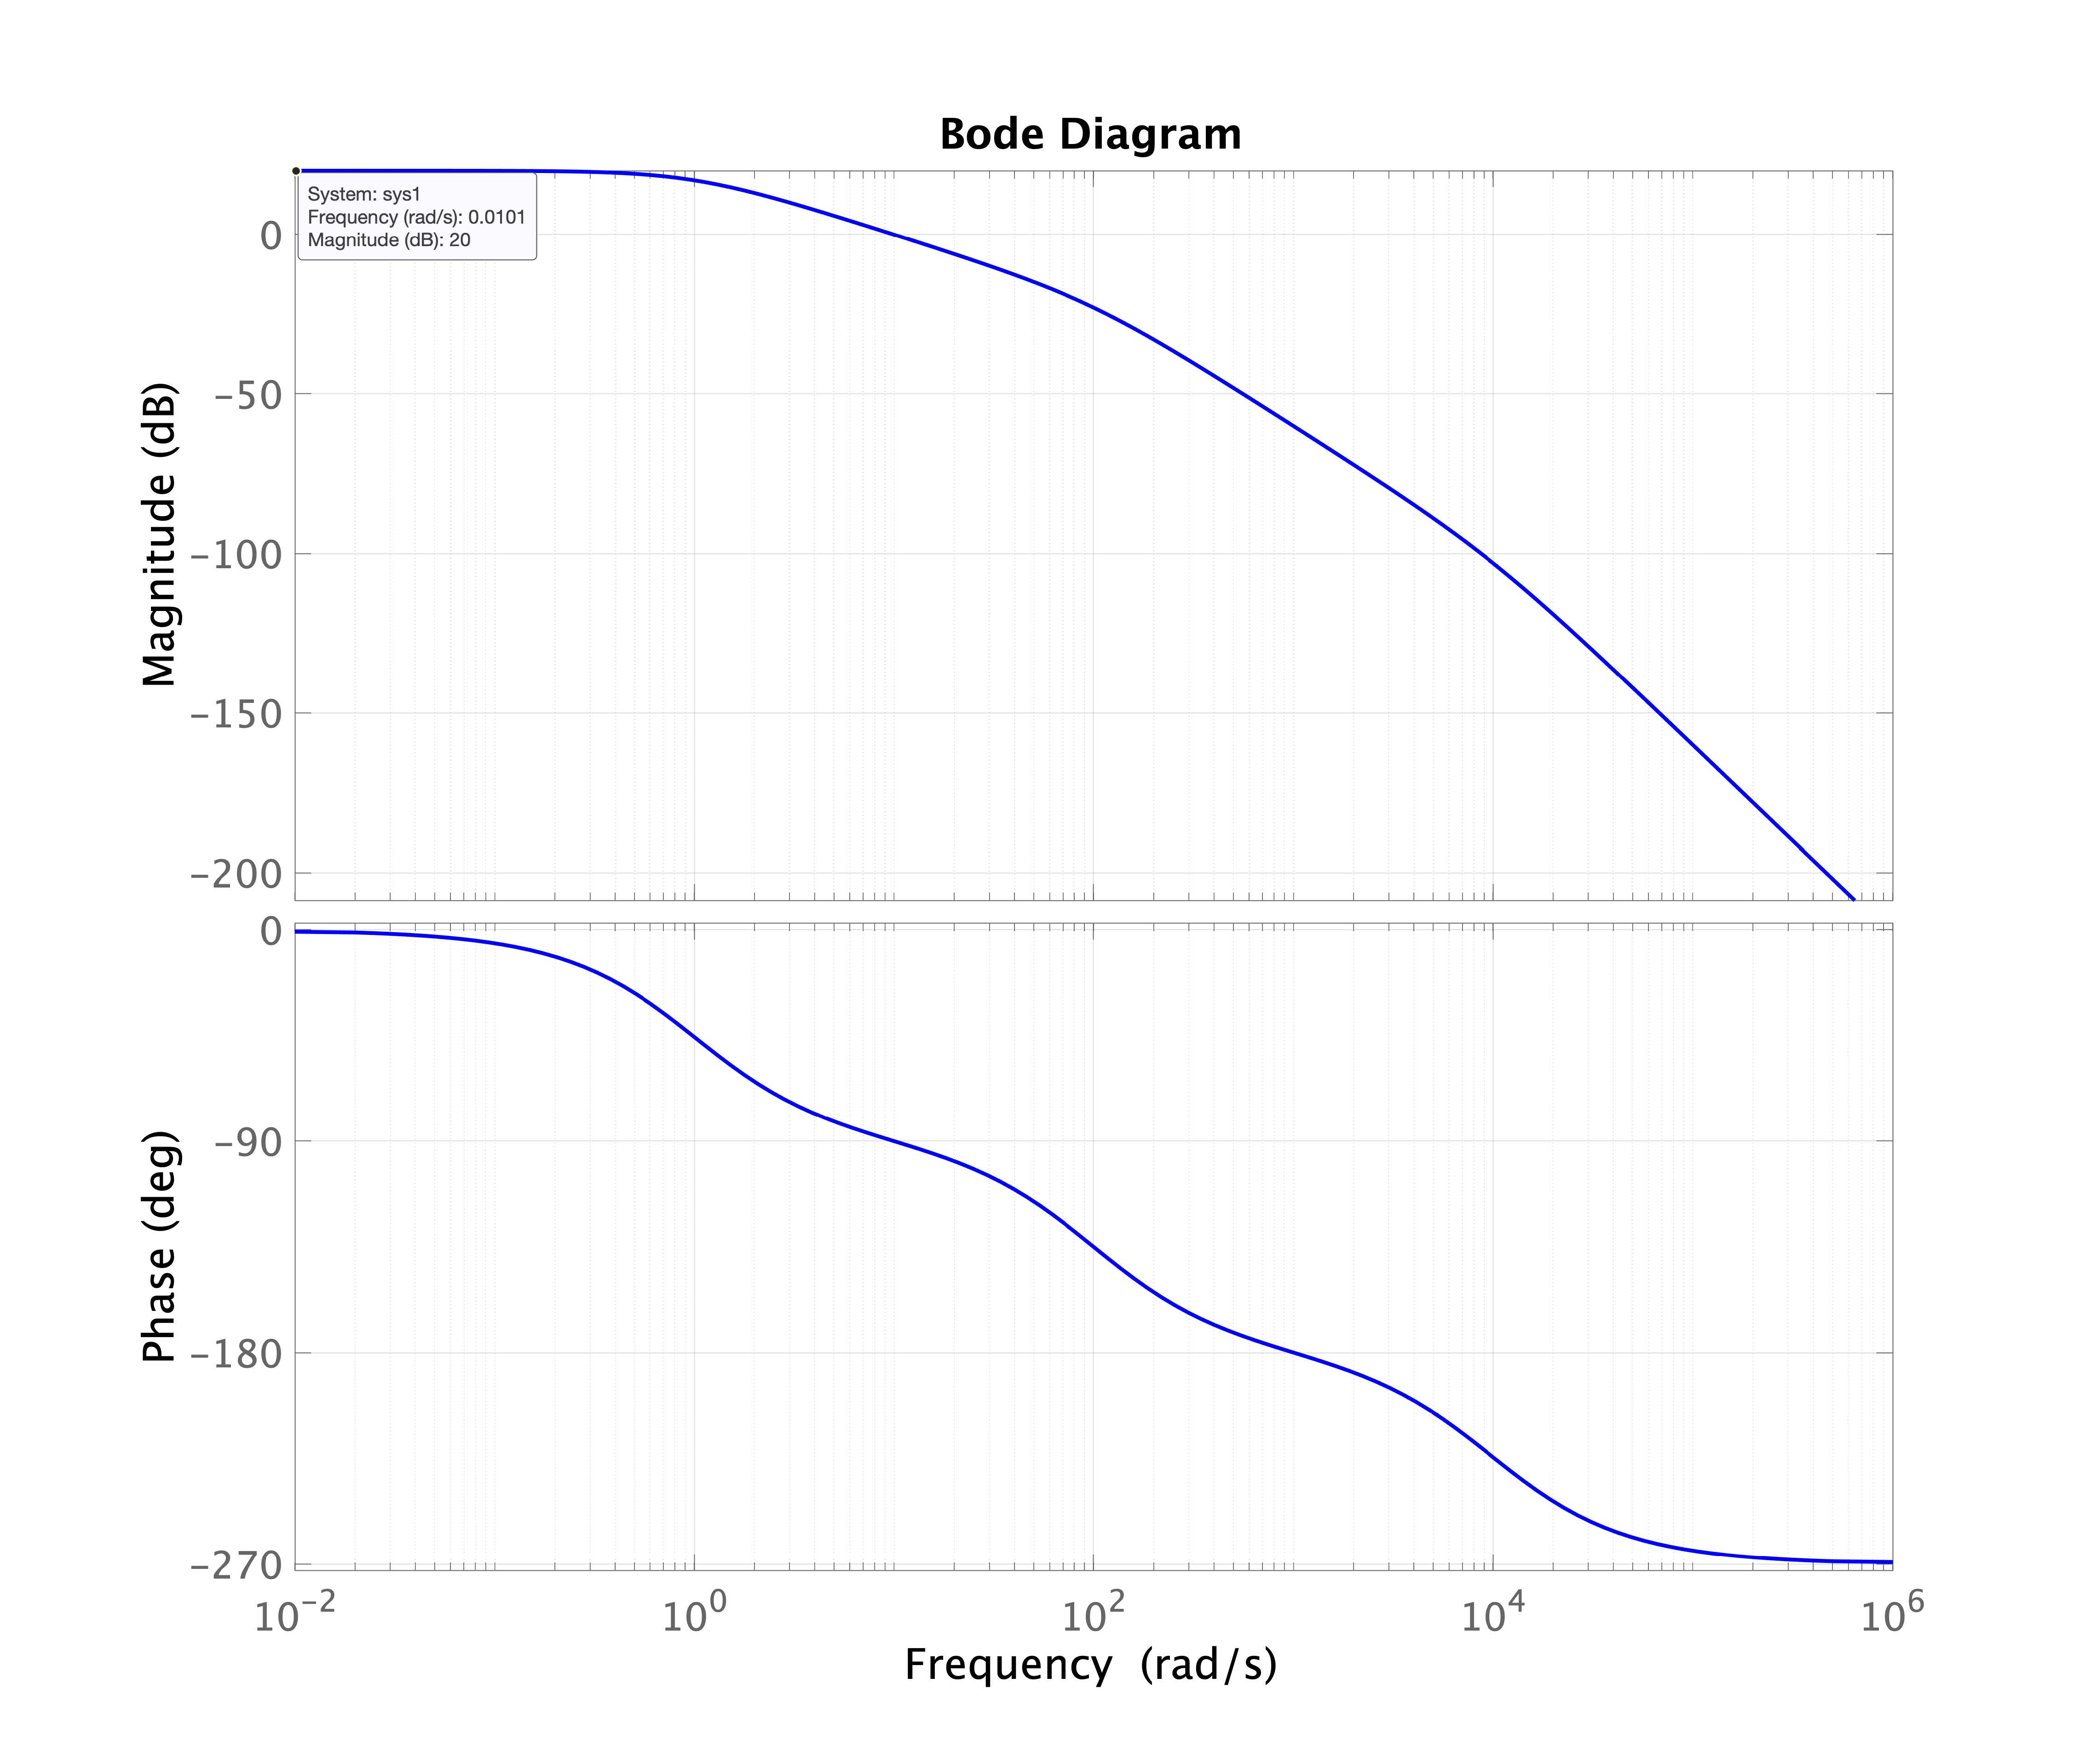
\includegraphics[width=0.5\textwidth]{figs/pblm3a.jpg}
\end{figure}

\subsubsection{Gain, Poles, and Zeros:}
\begin{enumerate}
	\item \textbf{Gain:}  $20$ db = 10
	\item \textbf{Poles:}
	\begin{enumerate}
		\item $10^{0} = 1$ rad/s
		\item $10^{2} = 100$ rad/s
		\item $10^{4} = 10,000$ rad/s
	\end{enumerate}
	\item Zeros: (NA)
\end{enumerate}

\textbf{Transfer Function:}\[
	H(s) = \cfrac{10}{
		\qty(1 + \frac{s}{1}) \qty(1 + \frac{s}{100}) \qty(1 + \frac{s}{10000})
		}
\]

\subsubsection{Cross-over Frequency:}
\begin{enumerate}
	\item $\omega_c = 10^{1} = 10$ rad/s
	\item $\omega_{180} = 10^{3} = 100$ rad/s
\end{enumerate}



\newpage
\subsection{Bode Plot 2:}
\begin{figure}[ht]
	\centering
	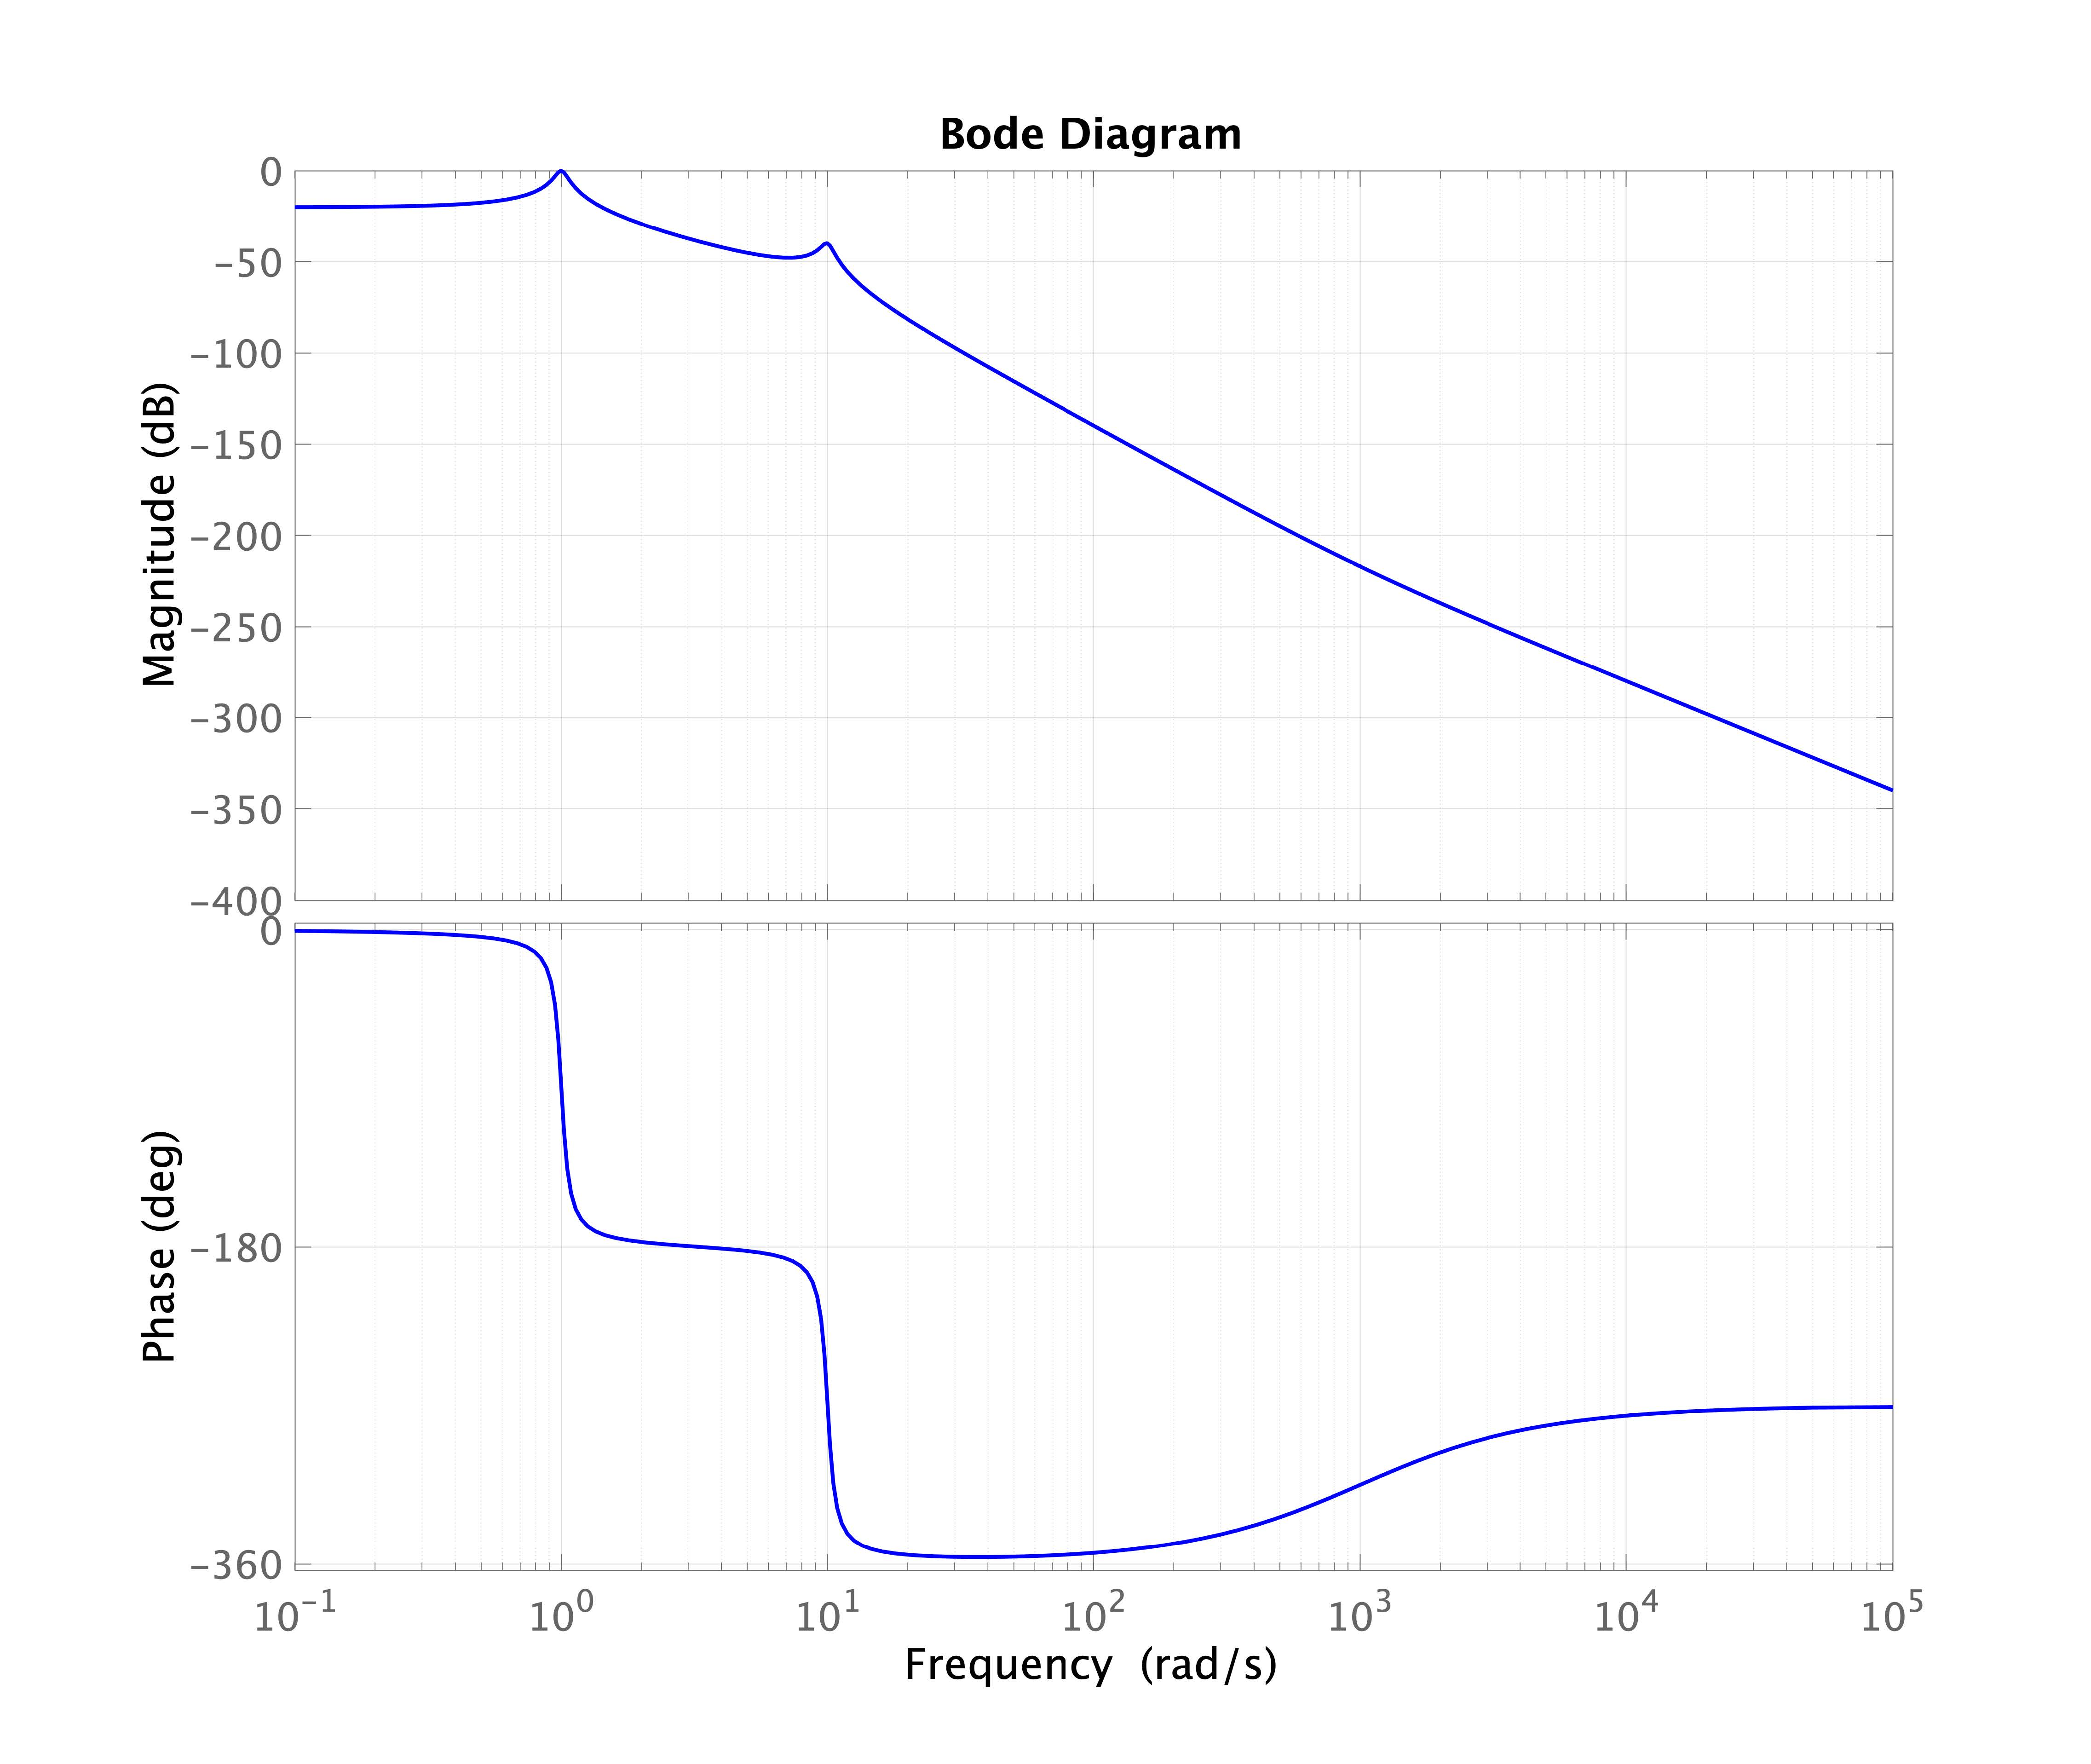
\includegraphics[width=0.5\textwidth]{figs/pblm3b.jpg}
	\caption{Bode Plot 2}
\end{figure}

\subsubsection{Gain, Poles, and Zeros:}
\begin{enumerate}
	\item \textbf{Gain:}  $-20$ db = $\frac{1}{10}$
	\item \textbf{Poles:}
	\begin{enumerate}
		\item $10^{0} = 1$ rad/s (complex)
		\item $10^{1} = 10$ rad/s (complex)
	\end{enumerate}
	\item Zeros:
	\begin{enumerate}
		\item $10^{3} = 1,000$ rad/s
	\end{enumerate}
\end{enumerate}

\subsubsection{Transfer Function:}\[
	H(s) = \cfrac{
			(1 + \frac{s}{1000})
		}{
			10 \qty(
				\frac{1}{1}\qty(s^2 + 2(\frac{1}{10})(1)s + (1)^2)
			) \qty(
				\frac{1}{10}\qty(s^2 + 2(\frac{1}{10})(10)s + (10)^2)
			)
		} = \cfrac{
			(s+1000)
		}{
			\qty(s^2 + 0.2 s + 1) \qty(s^2 + 2s + 100)
		}
\]
Assuming a Q-factor of around 10 to get the complex response.


\subsubsection{Cross-over Frequency:}
\begin{enumerate}
	\item $\omega_c = 10^{0} = 1$ rad/s
	\item $\omega_{180} = 10^{3} = 100$ rad/s
\end{enumerate}



\newpage
\section{Problem 4}
Consider the interconection of Problem 1 with the PI controller\[
	C(s) = \cfrac{10 (s+3)}{s}
\] and plant \[
	P(s) = \cfrac{-0.5(s^2 - 2000)}{(s-3)(s^2 + 50s + 1000)}
\]

\subsection{Is the feedback system stable? Why?}
\begin{align*}
	\cfrac{C(s) P(s)} {1 + C(s) P(s)}
		&= \cfrac{
			\cfrac{10 (s+3)}{s} \cfrac{-0.5(s^2 - 2000)}{(s-3)(s^2 + 50s + 1000)}
		}{
			1 + \cfrac{10 (s+3)}{s} \cfrac{-0.5(s^2 - 2000)}{(s-3)(s^2 + 50s + 1000)}
		}\\
		&\approx \cfrac{
			-5 s (s+3) (s-3) (s^2 - 2000) (s^2 + 50s + 1000)
		}{
			s (s-3) (s^2 + 11.73s + 73.9) (s^2 + 30.27s + 406) (s^2 + 50s + 1000)
		}
\end{align*}
Yes and No. 
Internally it is not fully stable since it has a pole/zero pair at $s=3$;
however, if we only care about TF after cancellations, then it is stable.

\subsection{Find phase and cross-over frequencies.}

\textbf{Problem:}
Use the Bode plot of the open loop transfer function $L(s) = C(s)P(s)$ to find the phase cross-over frequencies $\omega_0$ such that $L(j\omega_0) = 180\deg$. 
Use this information to compute the gain margin(s) of the feedback system. 
Check your answers using the \emph{allmargin} command in MATLAB.

\begin{figure}[ht]\label{fig:pblm4b}
	\centering
	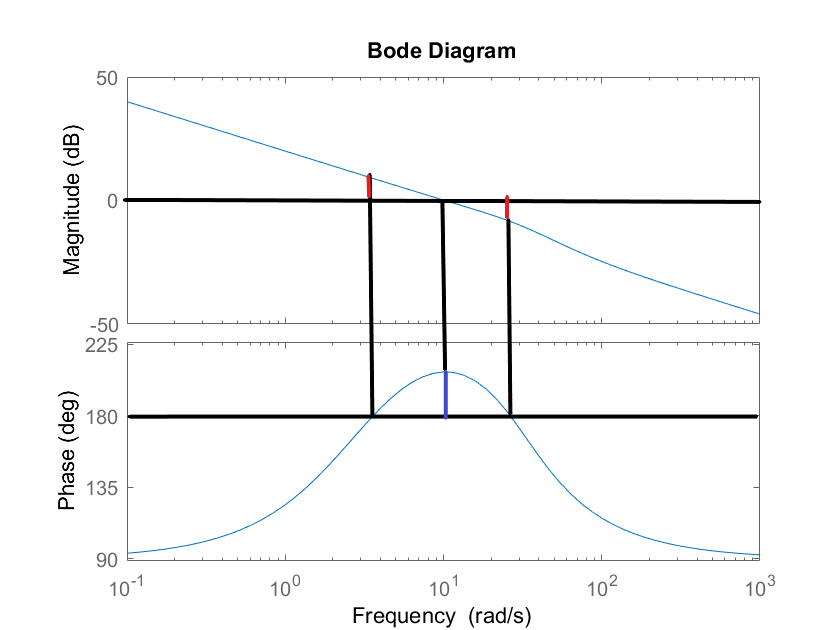
\includegraphics[width=0.7\textwidth]{figs/pblm4_L_bode.png}
	\caption{Open Loop Bode Plot of $L(S) = C(s) P(s)$}
\end{figure}

\textbf{Solution:}
As marked in the Bode Plot seen in \figurename \ \ref{fig:pblm4b}, 
the gain cross-over frequency is $\omega_{c} = 10$ resulting in a phase margin around $25\deg$.
Similarly, the phase cross-over occurs around $\omega_{180} = 4$ or $\omega_{180} = 25$, resulting in gain margins of around $\pm 10$ dB or around $g_0 = 0.3$ and $g_0 = 3$ respectively.

Verification with \emph{allmargin} resulted in similar and likely more precise and accurate results:
\begin{enumerate}
	\item Gain Margin(s)
	\begin{enumerate}
		\item $g_0 = 0.3585$ at $\omega_{180} =  3.5966$
		\item $g_0 = 2.6490$ at $\omega_{180} = 26.3797$
	\end{enumerate}
	\item Phase Margin
	\begin{enumerate}
		\item $PM = 27.5718$ at $\omega_{c} = 10.2049$
	\end{enumerate}
\end{enumerate}

\subsection{Gain Margin Closed-loop poles}
\textbf{Problem:} 
For each gain margin $g_0$ obtained in the previous part, construct the closed-loop using the perturbed loop transfer function $g_0 L(s)$ and verify that the closed-loop has poles at $\pm \omega_0$.

\textbf{Solution:}
\subsubsection{$g_0 = 0.3585$}
Let $g_0 = 0.3585$, \[
	g_0 L(s) =  \cfrac{
		-1.7927 (s+3) (s+44.72) (s-44.72)
	}{
	   s (s-3) (s^2 + 50s + 1000)
	}
\] and the closed-loop becomes \[
	H = \cfrac{ 
          -1.7927 (s-44.72) (s+44.72) (s+3)
	}{
		(s^2 + 0.0008164s + 12.93) (s^2 + 45.21s + 831.7)
	}
\] This has complex poles located at $-0.0004 \pm j 3.596$, which is essentially roots at $\pm j \omega_{180}$.


\subsubsection{$g_0 = 2.6490$}
Let $g_0 = 2.6490$, \[
	g_0 L(s) =  \cfrac{
		-13.245 (s+3) (s+44.72) (s-44.72)
	}{
	   s (s-3) (s^2 + 50s + 1000)
	}
\] and the closed-loop becomes \[
	H = \cfrac{ 
		-13.245 (s+3) (s+44.72) (s-44.72)
	}{
		(s+29.94) (s+3.814) (s^2 + 0.003402s + 696)
	}
\] This has complex poles located at $-0.0017 \pm j 26.3818$, which is essentially roots at $\pm j \omega_{180}$.

\subsection{$\norm{S-T}_\infty$}
\textbf{Problem:}
Compute $\norm{S-T}_\infty$ and the corresponding frequency $\omega_{p}$ where the peak gain of $S-T$ is achieved.

\textbf{Solution:} 

Sensitivity TF: \[
	S(s) = \frac{1}{1+PC}
		= \cfrac{
			s (s-3) (s^2 + 50s + 1000)
		}{
			(s^2 + 11.73s + 73.9) (s^2 + 30.27s + 406)
		}
\]

Complementary Sensitivity TF: \[
	T(s) = \frac{PC}{1+PC}
		= \cfrac{
			-5 s (s-44.72) (s+44.72) (s+3) (s-3) (s^2 + 50s + 1000)
		}{
			s (s-3) (s^2 + 11.73s + 73.9) (s^2 + 30.27s + 406) (s^2 + 50s + 1000)
		}
\]

$S(s)-T(s)$: \[
	S(s)-T(s) = \cfrac{
		s (s-10.45) (s-3) (s+2.059) (s^2 + 11.73s + 73.9) (s^2 + 30.27s + 406) (s^2 + 50s + 1000) (s^2 + 60.4s + 1394)
		}{
			s (s-3) (s^2 + 11.73s + 73.9)^2 (s^2 + 30.27s + 406)^2 (s^2 + 50s + 1000)
		}
\]\[
	= \cfrac{
		(s-10.45) (s+2.059) (s^2 + 60.4s + 1394)
		}{
			(s^2 + 11.73s + 73.9) (s^2 + 30.27s + 406)
		}
\]

Results:\[
	\norm{S-T}_\infty = 4.0763
\]\[
	\omega_{p} = 10.0798
\]

\subsection{Symmetric Disk Margin}
\textbf{Problem:}
What is the symmetric disk margin m for this plant and controller? 
Verify your answer using \emph{dm = diskmargin(P*C)}. 
Note that the \emph{diskmargin} command uses the convention \emph{m = dm.DiskMargin / 2}.

\textbf{Solution:}
By the Symmetric Disk Margin theorem, the disk margin defined for \[
	\alpha \in \text{Disk}\qty(\frac{1-m}{1+m},\frac{1+m}{1-m})
\] is the region that $C(s)$ stabilizes $\alpha P(s)$ for $m < 1$ satisfying\[
	\norm{S-T}_\infty \leq \frac{1}{m}
\] Therefore, \[
	\overline{m}_{st} = \cfrac{1}{\norm{S-T}_\infty} 
	= \cfrac{1}{4.0763} = 0.453
\]

\subsection{$\alpha$ on Disk boundary}
\textbf{Problem:}
Construct an $\alpha$ on the boundary of Disk \[
	\text{Disk}\qty(\frac{1-m}{1+m},\frac{1+m}{1-m})
\] such that the perturbed closed-loop \[
	S_\alpha = \frac{1}{1 + \alpha L(s)}
\] has a pole at $j\omega_p$. 
Verify your construction by forming $S_\alpha$ and demonstrating that it has a pole at $j \omega_p$.
Hint: Assume $\norm{S-T}_\infty = \frac{1}{m}$ at frequency $\omega_p$. 
Then there exists a complex number $S(j\omega_p) - T(j\omega_p) = \frac{1}{z}$ where $\abs{z} = m$.
Algebraically show that \[
	\alpha = \frac{1 + z}{1-z}
\] satisfies $1 + \alpha L(j\omega_p) = 0$ and this $\alpha$ is in the symmetric disk defined by $m$.

\textbf{Solution:}
$\alpha$ can be constructed by first finding $z_0 = \frac{1}{S(j\omega_p)-T(j\omega_p)}$, 
calculating $z = m * \frac{z_0}{\abs{z_0}}$, 
and then finding $\alpha = \frac{1+z}{1-z}$.

As demonstrated in MATLAB, this results in $\alpha = 0.8760 - j 0.4572$.
This is then verified as
\begin{align*}
	1 + \alpha L(j\omega_p) 
	&\approx (0.8760 - j 0.4572) \cfrac{
			-5 (j 10.0798+3) (j 10.0798+44.72) (j 10.0798-44.72)
		}{
			(j 10.0798) (j 10.0798-3) ((j 10.0798^2 + 50(j 10.0798) + 1000)
		}\\
	&= -2.7529e-08 - j 1.2029e-06\\
	&\approx 0
\end{align*}



\newpage
\appendix
\section{MATLAB Code:}\label{apx:matlab}
See attached.
Additionally, all the code I write in this course can be found on my GitHub repository:\\
\href{https://github.com/jonaswagner2826/MECH6323}{https://github.com/jonaswagner2826/MECH6323}

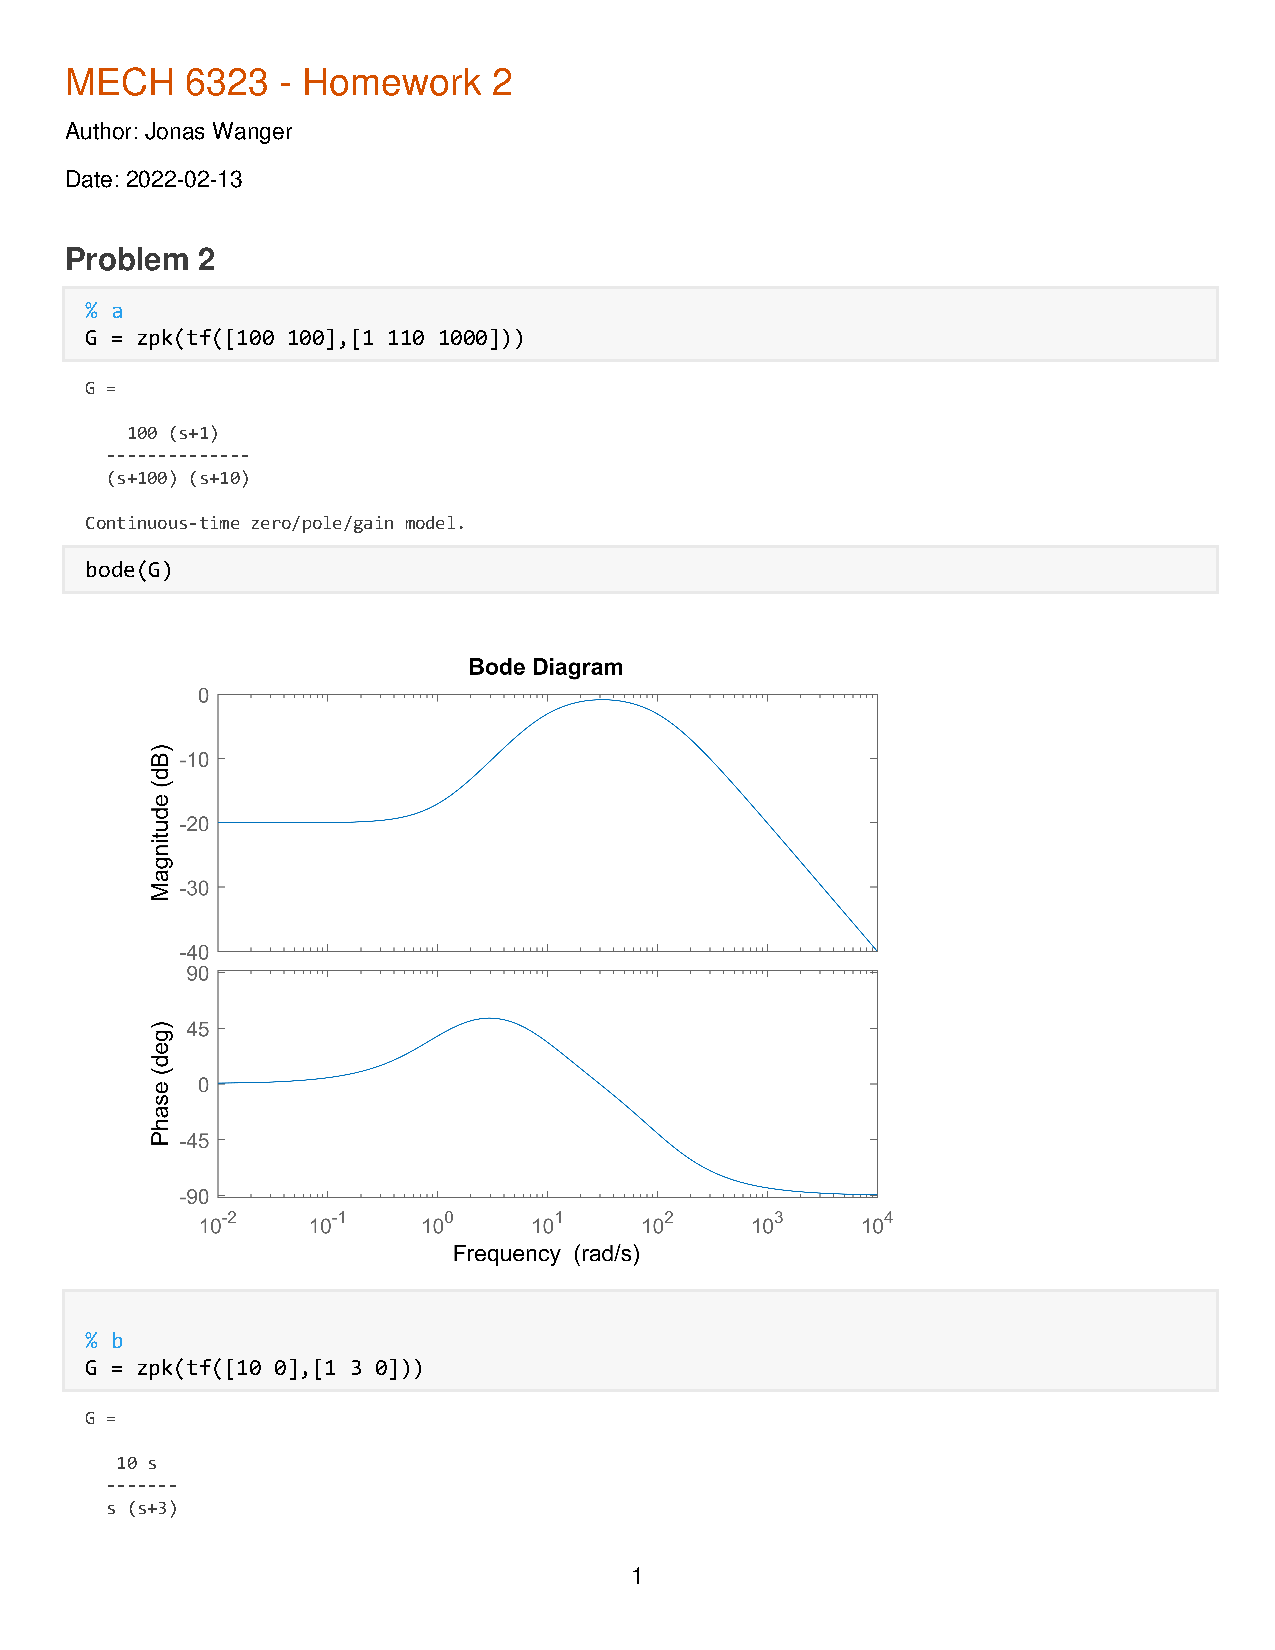
\includepdf[pages=-]{MECH6323_HW02.pdf}




\end{document}
